\documentclass[10pt,a4paper]{article}
\usepackage[utf8]{inputenc}
\usepackage[T1]{fontenc}
\usepackage{lmodern}
\usepackage[margin=10mm]{geometry}
\usepackage{amsmath,amssymb,amsfonts}
\usepackage{booktabs}
\usepackage{graphicx}
\usepackage{xcolor}
\usepackage{hyperref}

\definecolor{navy}{HTML}{1B365D}
\definecolor{slate}{HTML}{4A5568}
\hypersetup{colorlinks=true,linkcolor=navy,urlcolor=navy,citecolor=navy}
\sloppy\setlength{\textfloatsep}{5pt}\setlength{\floatsep}{5pt}\setlength{\intextsep}{5pt}\renewcommand{\topfraction}{0.95}\renewcommand{\bottomfraction}{0.95}\renewcommand{\textfraction}{0.04}\renewcommand{\floatpagefraction}{0.9}

\title{\vspace{-10mm}{\bfseries\color{navy}Kovariáns hatásjelöltek és nemlokális statikus konzisztenciavizsgálatok az Idővonzási Törvényhez (\texttt{50aa2db0} feladat)}\\[4pt]
{\normalsize Bilaterális top-hat mozgásegyenlet vs.\ árnyékolt Helmholtz--Yukawa-hatás, a statikus érintőoperátor konzisztenciája és az óracsatolás (H0 vs.\ H1)}}
\author{\textbf{Szabolcsi Dávid} \quad (ORCID: \href{https://orcid.org/0009-0005-6300-074X}{\texttt{0009-0005-6300-074X}})\\
{\small Független kutató $\cdot$ Licenc: CC BY-NC 4.0 $\cdot$ Dátum: 2026-10-24}}
\date{}

\begin{document}
\maketitle
\vspace{-6mm}

\begin{abstract}\noindent
Ebben az önálló matematikai és numerikus tanulmányban az \texttt{50aa2db0} feladatot vizsgálom: kovariáns hatásjelölteket és nemlokális statikus konzisztenciavizsgálatokat az Idővonzási Törvényhez (TAL), a 3D gömbi top-hat megfogalmazásra (DOI \texttt{10.5281/zenodo.23497128}), a kétkarú laboratóriumi programra (DOI \texttt{10.5281/zenodo.23540741}), a kompakt objektumok TOV- és radiális stabilitási vizsgálatára (DOI \texttt{10.5281/zenodo.23602501}) és a V22 monográfiára (DOI \texttt{10.5281/zenodo.23604423}) építve. Először két kovariáns hatásjelöltet hasonlítok össze: \textbf{I.\ megfogalmazás} (nemlokális pozitív-definit bilaterális mag-hatás $\phi_L, \lambda_L$ segédmezőkkel) és \textbf{II.\ megfogalmazás} (lokális árnyékolt Helmholtz--Yukawa skalár-tenzor hatás, $(-L^2\nabla^2+1)\phi_L = \alpha_Y\gamma_L\rho_{\text{src}}$). Másodszor szimbolikusan megmutatom, hogy az algebrailag rekonstruált X-szektorra $\nabla_\mu(T^{\mu\nu}_{\text{matter}} + T^{\mu\nu}_X) = 0$ azonosan teljesül, és ezt elválasztom a numerikus maradékoktól (algebrai X-szektor kvadratúra $\lesssim 4\times 10^{-14}$; spline-alapú divergencia $\lesssim 2{,}7\times 10^{-5}$); emellett megoldok egy bilaterális reciprok erővel kiegészített, síkbeli kernelű fixpontos egyensúlyt (súlyozatlanul és lapse-súlyozva), valamint egy hatással konzisztens Yukawa-TOV-ágat. Harmadszor a V21-háttéren futtatott, a $\delta f_L[\delta\varepsilon, \xi]$ nemlokális perturbációt tartalmazó kvázi-dinamikus BVP-teszt kiválasztott ágának zérushelye az SLy $L=10\,\text{km}$ sorozaton $+6{,}97\times 10^{-5}\,\text{dex}$ (mass) és $+7{,}39\times 10^{-5}\,\text{dex}$ (gradient) távolságra van a $dM/d\rho_c = 0$ ponttól; ez a nemlokális statikus érintőoperátor konzisztenciáját mutatja. Mivel $\omega^2=0$-t a statikus linearizáció rögzíti, a zérushely invariáns a $W\to 4W$ tehetetlenség-skálázásra (numerikusan ellenőrizve); ez nem dinamikai bizonyíték a görbült téri ablak-variációra, amely nyitott kérdés marad. Negyedszer megmutatom, hogy a Dirac--Maxwell anyaghatás Jordan-metrikájának választása választ a \textbf{H0} és \textbf{H1} megfigyelési hipotézisek között a Szíriusz B és a $8558\,\text{kg}$-os gránitkamra esetén.
\end{abstract}

\section{Kovariáns hatás-megfogalmazások: bilaterális mag vs.\ árnyékolt Yukawa}
Ahhoz, hogy a rögzített, pozitív-definit $f_L(x) = \exp(-\phi_L(x)) \in (0,1]$ exponenciális törvényt ($\gamma_L = \alpha (G/c^2)L^2$, $\alpha=1$) ad-hoc háttér-könyvelés nélkül dinamikai variációs elvhez kapcsoljam, két explicit kovariáns hatást hasonlítok össze:
\begin{equation}
  S[g_{\mu\nu}, \phi_L, \lambda_L, \Psi_{\text{matter}}] = \int d^4x\sqrt{-g}\left[\frac{c^4}{16\pi G}R + \mathcal{L}_X(g_{\mu\nu}, \phi_L, \lambda_L) + \mathcal{L}_{\text{matter}}\!\left(\tilde{g}_{\mu\nu}[\phi_L], \Psi_{\text{matter}}\right)\right].
\end{equation}

\subsection{I.\ megfogalmazás: nemlokális pozitív-definit mag-hatás és bilaterális reciprocitás}
Az I.\ megfogalmazásban a $\phi_L(x)$ segédskalárt egy $\lambda_L(x)$ Lagrange-multiplikátor mező kapcsolja a folyadék $u^\mu$ négyes-sebességére ortogonális $\Sigma_u$ hiperfelületen ($h_{\mu\nu} = g_{\mu\nu} + u_\mu u_\nu/c^2$) vett térbeli top-hat átlaghoz:
\begin{equation}
  S_{\text{I},X}[\phi_L, \lambda_L, g_{\mu\nu}] = -\frac{c^4}{8\pi G \gamma_L}\int d^4x\sqrt{-g}\,\lambda_L(x)\!\left[\phi_L(x) - \gamma_L \int_{\Sigma_u} d^4y\sqrt{-g(y)}\,K_L(x,y)\,\rho_{\text{src}}(y)\right],
\end{equation}
ahol $K_L(x,y) = \delta(\tau_u(x)-\tau_u(y))\,\Theta(L - d_\Sigma(x,y))/V_L(x)$ az $L$ sugarú, $V_L = \frac{4}{3}\pi L^3$ saját-térfogatú pozitív-definit 3D gömbi mag. A $\lambda_L(x)$, $\phi_L(x)$ és $\rho_{\text{src}}(x)$ szerinti variáció az alábbi Euler--Lagrange-lezárást adja:
\begin{equation}
  \frac{\delta S}{\delta \lambda_L(x)} = 0 \implies \phi_L(x) = \gamma_L\bar{\rho}_L(x),\quad f_L(x) = e^{-\phi_L(x)}; \qquad
  \frac{\delta S}{\delta \phi_L(x)} = 0 \implies \lambda_L(x) = \frac{8\pi G\gamma_L}{c^4}\frac{\partial \mathcal{L}_{\text{eff}}}{\partial \phi_L}(x).
\end{equation}
Mivel $\rho_{\text{src}}(y)$ az $y$ szerinti integrál belsejében szerepel, a folyadéksűrűség $x$-beli variációja felcseréli az $x \leftrightarrow y$ integrációs változókat (\emph{bilaterális mag-reciprocitás}), és egy $V_{\text{recip}}(x) = \int d^3y\,K_L(y,x)\lambda_L(y)$ reciprok potenciállal egészíti ki az Euler-egyenletet. Statikus gömbszimmetrikus belső térben, ha a $T^\mu_{\;\nu}(X) = \text{diag}(-\varepsilon_X, P_{r,X}, P_{t,X}, P_{t,X})$ segédszektor veszi fel az ablak-feszültséget a $G^\mu_{\;\nu} = \frac{8\pi G}{c^4}(T^\mu_{\;\nu,\text{matter}} + T^\mu_{\;\nu,X})$ egyenlet jobb oldalán, míg a folyadékelemek kielégítik a $\nabla_\mu T^{\mu\nu}_{\text{matter}} = 0$ egyenletet ($P' = -(\varepsilon+P)\nu'$ geometrizált egységekben, $G=c=1$, $\nu = \Phi_{\text{eff}}/c^2$, $g_{tt}=-e^{2\nu}=-e^{2\Phi_{\text{eff}}/c^2}$), akkor a $\nabla_\mu G^\mu_{\;r} \equiv 0$ Bianchi-azonosság mindkét V21 módban egyértelműen rögzíti $T^\mu_{\;\nu}(X)$-et:
\begin{align}
  \textbf{Tömeg-mód } (m' = 4\pi r^2 f_L\varepsilon,\; \nu' = A_{\text{geo}}): &\quad \varepsilon_X = -(1-f_L)\varepsilon,\quad P_{r,X} = 0,\quad P_{t,X} = -\frac{r}{2}(1-f_L)\varepsilon\nu', \label{eq:mass_X}\\
  \textbf{Gradiens-mód } (m' = 4\pi r^2\varepsilon,\; \nu' = f_L A_{\text{geo}}): &\quad \varepsilon_X = 0,\quad P_{r,X} = -(1-f_L)\!\left(P + \frac{m}{4\pi r^3}\right),\; P_{t,X} = P_{r,X} + \frac{r}{2}\bigl(P'_{r,X} + P_{r,X}\nu'\bigr), \label{eq:grad_X}
\end{align}
ahol $A_{\text{geo}}(r) = (m + 4\pi r^3 P)/[r(r-2m)]$. A \texttt{SymPy}-ban elvégzett szimbolikus ellenőrzés (\texttt{conservation\_Residuals.json}) igazolja, hogy $\nabla_\mu T^\mu_{\;r}(\text{matter}) \equiv 0$ és $\nabla_\mu T^\mu_{\;r}(X) \equiv 0$ azonosságszerűen fennáll. Az 1.\ táblázatban és az 1(b).\ ábrán a \eqref{eq:mass_X}--\eqref{eq:grad_X} összefüggések kiértékelése a numerikus TOV-rácsokon ($L=10\,\text{km}$, $\log_{10}\rho_{0c}=15{,}0$) három különálló szintet ad (\texttt{conservation\_Residuals.json}): (i) szimbolikus azonosságok, maradék pontosan $0$; (ii) algebrai X-szektor kvadratúra-maradék $\max|\nabla_\mu T^\mu_{\;r}(X)|/|\rho_X\nu'| = 4{,}44\times 10^{-16}$ (mass) és $/|P'_{r,X}| = 4{,}39\times 10^{-14}$ (gradient); (iii) a numerikusan (spline-nal) differenciált háttér divergenciája $\max|\nabla_\mu T^\mu_{\;r}|/|P'| = 2{,}70\times 10^{-5}$ (mass) és $2{,}36\times 10^{-5}$ (gradient), amelyet $h(r)$ véges differenciás deriváltja határoz meg, nem a hatás.

\emph{Bilaterális reciprok erővel kiegészített, síkbeli kernelű fixpontos egyensúly.} Ha $\lambda_L$-t a folyadékba olvasztjuk $\mathcal{L}_{\text{fluid}}(n,\phi_L) = -f_L(\phi_L)\,\varepsilon(n)$ alakban, és $\varepsilon$-t explicit módon és a magon belül is variáljuk, akkor $V_{\text{eff}}(x) = f_L(x) - \gamma_L\!\int K_L(y,x) f_L(y)\varepsilon(y)\,d^3y$ és a módosított egyensúly $dh/dr = -A(r) - dV_{\text{recip}}/dr$, $V_{\text{recip}} = \ln V_{\text{eff}}$. Ezt önkonzisztens fixpontként oldom meg (\texttt{bilateral\_eom} sorok az 1.\ táblázatban); eltér az algebrailag lezárt V21 mass-módtól. Az $N=e^\nu$ lapse-szal súlyozott $\int dV\,N f_L\varepsilon$ variációja (rögzített mag és metrika mellett) $V_{\text{eff},N}(x)=f_L-\frac{\gamma_L}{N(x)}\!\int dV_y\,N(y)K(y,x)f_L\varepsilon$, amelyet a lapse-egyenletben $P_{\text{matter}}=f_LP$ mellett oldok meg (\texttt{bilateral\_lapse\_weighted} sorok; kétcellás próba $N=(1;0{,}8)$, $\varepsilon=(1;2)$, $\gamma=0{,}1$: $(0{,}74882;0{,}72084)$, súlyozatlanul $0{,}73160$). A kovariáns lezáráshoz még a mag és a térfogatelem metrikus variációja szükséges; egyik sor sem a (2) hatás EL-megoldása.

\subsection{II.\ megfogalmazás: lokális árnyékolt skalár-tenzor (Helmholtz--Yukawa) hatás}
A II.\ megfogalmazásban a nemlokális integrálmagot lokális kanonikus árnyékolt skalárhatással helyettesítem:
\begin{equation}
  \mathcal{L}_\phi = -\frac{c^4}{8\pi G \tilde{\alpha}_L}\!\left[\frac{1}{2}g^{\mu\nu}\nabla_\mu\phi_L\nabla_\nu\phi_L + \frac{1}{2L^2}\phi_L^2\right], \quad \left(-\Box_g + \frac{1}{L^2}\right)\phi_L = \frac{4\pi G}{c^2}\alpha_{\text{std}}\,\rho_{\text{src}} \iff (-L^2\nabla^2+1)\phi_L = \alpha_Y\gamma_L\rho_{\text{src}}.
\end{equation}
Statikus gömbi rendszerben a $-\frac{1}{r^2}\frac{d}{dr}(r^2\phi_L') + L^{-2}\phi_L = \frac{4\pi G}{c^2}\alpha_{\text{std}}\rho_{\text{src}}$ ($\alpha_Y = 4\pi\alpha_{\text{std}}$) radiális Helmholtz-operátor egzakt, pozitív-definit Green-függvényes megoldása
\begin{equation}
  \phi_L^{\text{Yuk}}(r) = \alpha_Y\,\frac{G}{c^2}\int_0^{R_*} dr'\,\frac{r' L}{r}\,\sinh\!\frac{r_<}{L}\,e^{-r_>/L}\rho_{\text{src}}(r'), \qquad \phi_L^{\text{Yuk}}(0) = \alpha_Y\,\frac{G}{c^2}\int_0^{R_*} r' e^{-r'/L}\rho_{\text{src}}(r')\,dr',
\end{equation}
a $\delta S_\phi/\delta g^{\mu\nu}$ variáció pedig a lokális kovariáns $T_{\mu\nu}^{(\phi)} = \frac{c^4}{8\pi G\tilde{\alpha}_L}\bigl[\nabla_\mu\phi_L\nabla_\nu\phi_L - \frac{1}{2}g_{\mu\nu}\bigl((\nabla\phi_L)^2 + L^{-2}\phi_L^2\bigr)\bigr]$ feszültség-energia tenzort szolgáltatja. (\texttt{SymPy}: \texttt{sym\_yukawa\_center\_limit\_residual} $=0$, nincs többlet $L$-faktor). Az egységre normált mag $\alpha_Y = 1$-nek, azaz $\alpha_{\text{std}} = 1/(4\pi)\approx 0{,}0796$-nak felel meg, ami visszaadja a homogén top-hat határesetet ($\phi_L = \gamma_L\rho_{\text{src}}$); az $\alpha_Y = 1/3$ ($\alpha_{\text{std}} = 1/(12\pi)$) a térfogatra illesztett változat. Mindkét normálás explicit szerepel a \texttt{closure\_tov\_comparison.csv}-ben (\texttt{alpha\_Y\_unit}, \texttt{alpha\_std\_poisson}). A \texttt{yukawa\_flat\_phenom\_Tphi} sorok síkbeli Yukawa-mezővel és hozzáadott skalárfeszültséggel számolt fenomenológiai TOV-modellt adnak. A \texttt{yukawa\_action\_el} sorok az $\mathcal{L}=-[(\nabla\phi)^2+\phi^2/L^2]/(2\alpha_Y)-f_L\varepsilon$ hatásból következnek ($G=c=1$; \texttt{SymPy}: \texttt{sym\_yukawa\_el\_source\_factor} és \texttt{\_hydrostatic} maradék $=0$): $B\phi''+(2B/r+B\nu'+B'/2)\phi'-\phi/L^2=-\alpha_Y f_L\varepsilon$, $B=1-2m/r$, $P_{\text{matter}}=f_LP$, $h'=-\nu'+\phi'$, $\rho_\phi=(B\phi'^2+\phi^2/L^2)/(2\alpha_Y)$, külső illesztés $\phi'(R)=-(1/R+1/L)\phi(R)$; a $\Delta M_{\phi,\text{ext}}$ külső farok külön szerepel (SLy, $L=10$ km: $3{,}4\times 10^{-3}\,M_\odot$ $\log_{10}\rho_{0c}=15$-nél, $9{,}0\times 10^{-3}\,M_\odot$ $M_{\max}$-nál). Az 1.\ táblázat és a 2.\ ábra az I.\ és II.\ megfogalmazást hasonlítja össze SLy, APR4 és H4 állapotegyenletekre.

\begin{table}[ht!]
\centering
\caption{Neutroncsillag TOV-sorozatok összehasonlítása az I.\ megfogalmazás (3D gömbi top-hat) és a II.\ megfogalmazás (árnyékolt Helmholtz--Yukawa, $\alpha_Y=1$ és $\alpha_Y=1/3$) szerint SLy, APR4 és H4 állapotegyenletekre (\texttt{closure\_tov\_comparison.csv}).}
\vspace{2pt}
\resizebox{\linewidth}{!}{%
\begin{tabular}{@{}lllcrrrrr@{}}
\toprule
EOS & $L$ [km] & Mód & Hatás-mag & $M_{\max}$ [$M_\odot$] & $R(M_{\max})$ [km] & $\log_{10}\rho_{0c,\text{turn}}$ & $R_{1.4}$ [km] & $f_L(0)\;|\;f_L(R_*)$ ($10^{15}$-nél) \\
\midrule
SLy  & 0.0  & GR       & Nincs ($f_L\equiv 1$)           & 2.04841 & 9.9756  & 15.30242 & 11.7061 & $1.000000 \;|\; 1.000000$ \\
SLy  & 1.0  & mass     & I.\ megf.\ (Top-Hat)            & 2.04974 & 9.9785  & 15.30282 & 11.7091 & $0.999169 \;|\; 0.999991$ \\
SLy  & 1.0  & mass     & II.\ megf.\ (Yukawa $\alpha_Y=1$) & 2.04964 & 9.9784  & 15.30278 & 11.7090 & $0.999199 \;|\; 0.999947$ \\
SLy  & 10.0 & mass     & I.\ megf.\ (Top-Hat)            & 2.09822 & 10.2029 & 15.30814 & 11.8703 & $0.950477 \;|\; 0.987551$ \\
SLy  & 10.0 & gradient & I.\ megf.\ (Top-Hat)            & 2.10848 & 10.0182 & 15.29876 & 11.7920 & $0.950680 \;|\; 0.987433$ \\
SLy  & 10.0 & mass     & II.\ megf.\ (Yukawa $\alpha_Y=1$) & 2.06707 & 10.0523 & 15.30566 & 11.7689 & $0.983728 \;|\; 0.994497$ \\
SLy  & 10.0 & gradient & II.\ megf.\ (Yukawa $\alpha_Y=1$) & 2.07112 & 9.9952  & 15.30050 & 11.7417 & $0.983762 \;|\; 0.994493$ \\
SLy  & 10.0 & mass     & II.\ megf.\ (Yukawa $\alpha_Y=1/3$)& 2.05456 & 10.0008 & 15.30349 & 11.7270 & $0.994576 \;|\; 0.998170$ \\
SLy  & 1.0 & mass & Bilaterális EOM & 2.04275 & 9.9615 & 15.30412 & 11.6744 & $0.999176 \;|\; 0.999990$ \\
SLy  & 10.0 & mass & Bilaterális EOM & 1.93214 & 9.5299 & 15.37713 & 10.9416 & $0.957872 \;|\; 0.988372$ \\
SLy  & 10.0 & mass & Bilat.\ lapse-súly. & 1.90217 & 9.5338 & 15.38661 & 10.9048 & $0.958539 \;|\; \text{--}$ \\
SLy  & 10.0 & mass & Yukawa síkb.\ fen. & 2.06211 & 10.0210 & 15.30422 & 11.7449 & $0.983754 \;|\; 0.994496$ \\
SLy  & 1.0 & mass & Yukawa hatás-EL & 2.04688 & 9.9687 & 15.30316 & 11.6935 & $0.999198 \;|\; 0.999956$ \\
SLy  & 10.0 & mass & Yukawa hatás-EL & 2.03583 & 9.9038 & 15.31684 & 11.5456 & $0.981575 \;|\; 0.993556$ \\
\midrule
APR4 & 0.0  & GR       & Nincs ($f_L\equiv 1$)           & 2.18800 & 9.8997  & 15.28232 & 11.3197 & $1.000000 \;|\; 1.000000$ \\
APR4 & 10.0 & mass     & I.\ megf.\ (Top-Hat)            & 2.24152 & 10.1359 & 15.28796 & 11.4757 & $0.948546 \;|\; 0.986533$ \\
APR4 & 10.0 & gradient & I.\ megf.\ (Top-Hat)            & 2.24877 & 9.9482  & 15.27761 & 11.3937 & $0.948803 \;|\; 0.986420$ \\
APR4 & 10.0 & mass     & II.\ megf.\ (Yukawa $\alpha_Y=1$) & 2.20777 & 9.9824  & 15.28512 & 11.3793 & $0.983526 \;|\; 0.994183$ \\
APR4 & 10.0 & mass & Bilaterális EOM & 2.08816 & 9.6262 & 15.34020 & 10.7328 & $0.956923 \;|\; 0.987475$ \\
APR4 & 10.0 & mass & Bilat.\ lapse-súly. & 2.05956 & 9.6246 & 15.35118 & 10.7038 & $0.957732 \;|\; \text{--}$ \\
\midrule
H4   & 0.0  & GR       & Nincs ($f_L\equiv 1$)           & 2.01385 & 11.6993 & 15.20909 & 13.9522 & $1.000000 \;|\; 1.000000$ \\
H4   & 10.0 & mass     & I.\ megf.\ (Top-Hat)            & 2.05990 & 11.8833 & 15.21776 & 14.0952 & $0.951154 \;|\; 0.989702$ \\
H4   & 10.0 & gradient & I.\ megf.\ (Top-Hat)            & 2.06963 & 11.7036 & 15.21068 & 14.0267 & $0.951249 \;|\; 0.989545$ \\
H4   & 10.0 & mass     & II.\ megf.\ (Yukawa $\alpha_Y=1$) & 2.03060 & 11.7635 & 15.21307 & 14.0096 & $0.982635 \;|\; 0.994798$ \\
H4   & 10.0 & mass & Bilaterális EOM & 1.80990 & 10.6968 & 15.33477 & 12.7249 & $0.956381 \;|\; 0.990180$ \\
H4   & 10.0 & mass & Bilat.\ lapse-súly. & 1.78279 & 10.7415 & 15.34078 & 12.6856 & $0.956941 \;|\; \text{--}$ \\
\bottomrule
\end{tabular}}
\end{table}

\begin{figure}[ht!]
\centering
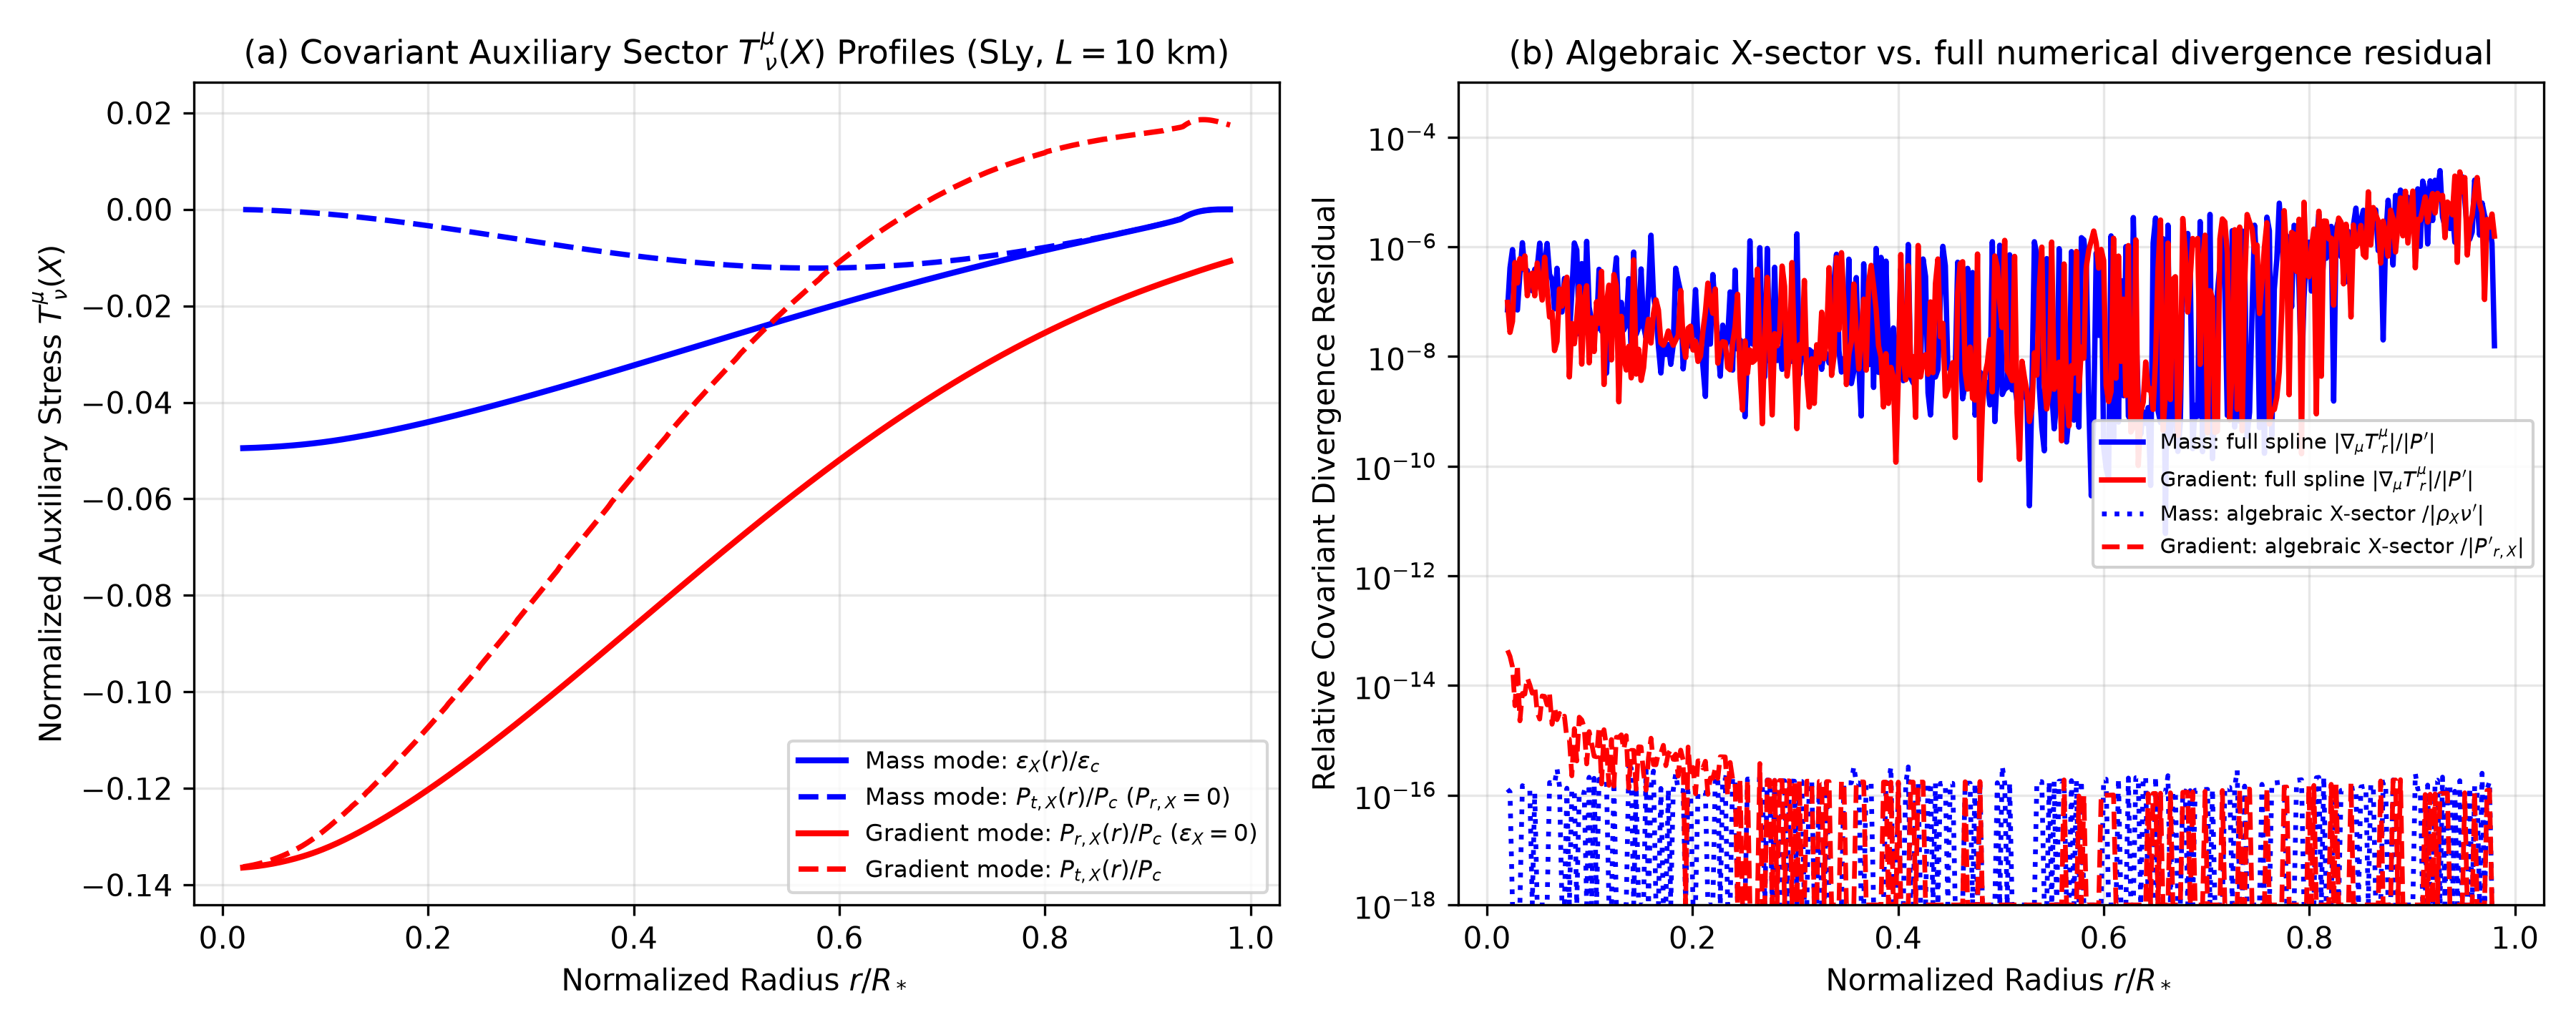
\includegraphics[width=0.66\linewidth]{fig3_conservation_check.png}\vspace{-3mm}
\caption{(a) A $T^\mu_{\;\nu}(X)$ segédszektor-komponensek és (b) a $|\nabla_\mu T^\mu_{\;r}|/|P'|$ relatív kovariáns divergencia-reziduálok SLy állapotegyenletre $L=10\,\text{km}$, $\log_{10}\rho_{0c}=15{,}0$ mellett.}
\end{figure}

\begin{figure}[ht!]
\centering
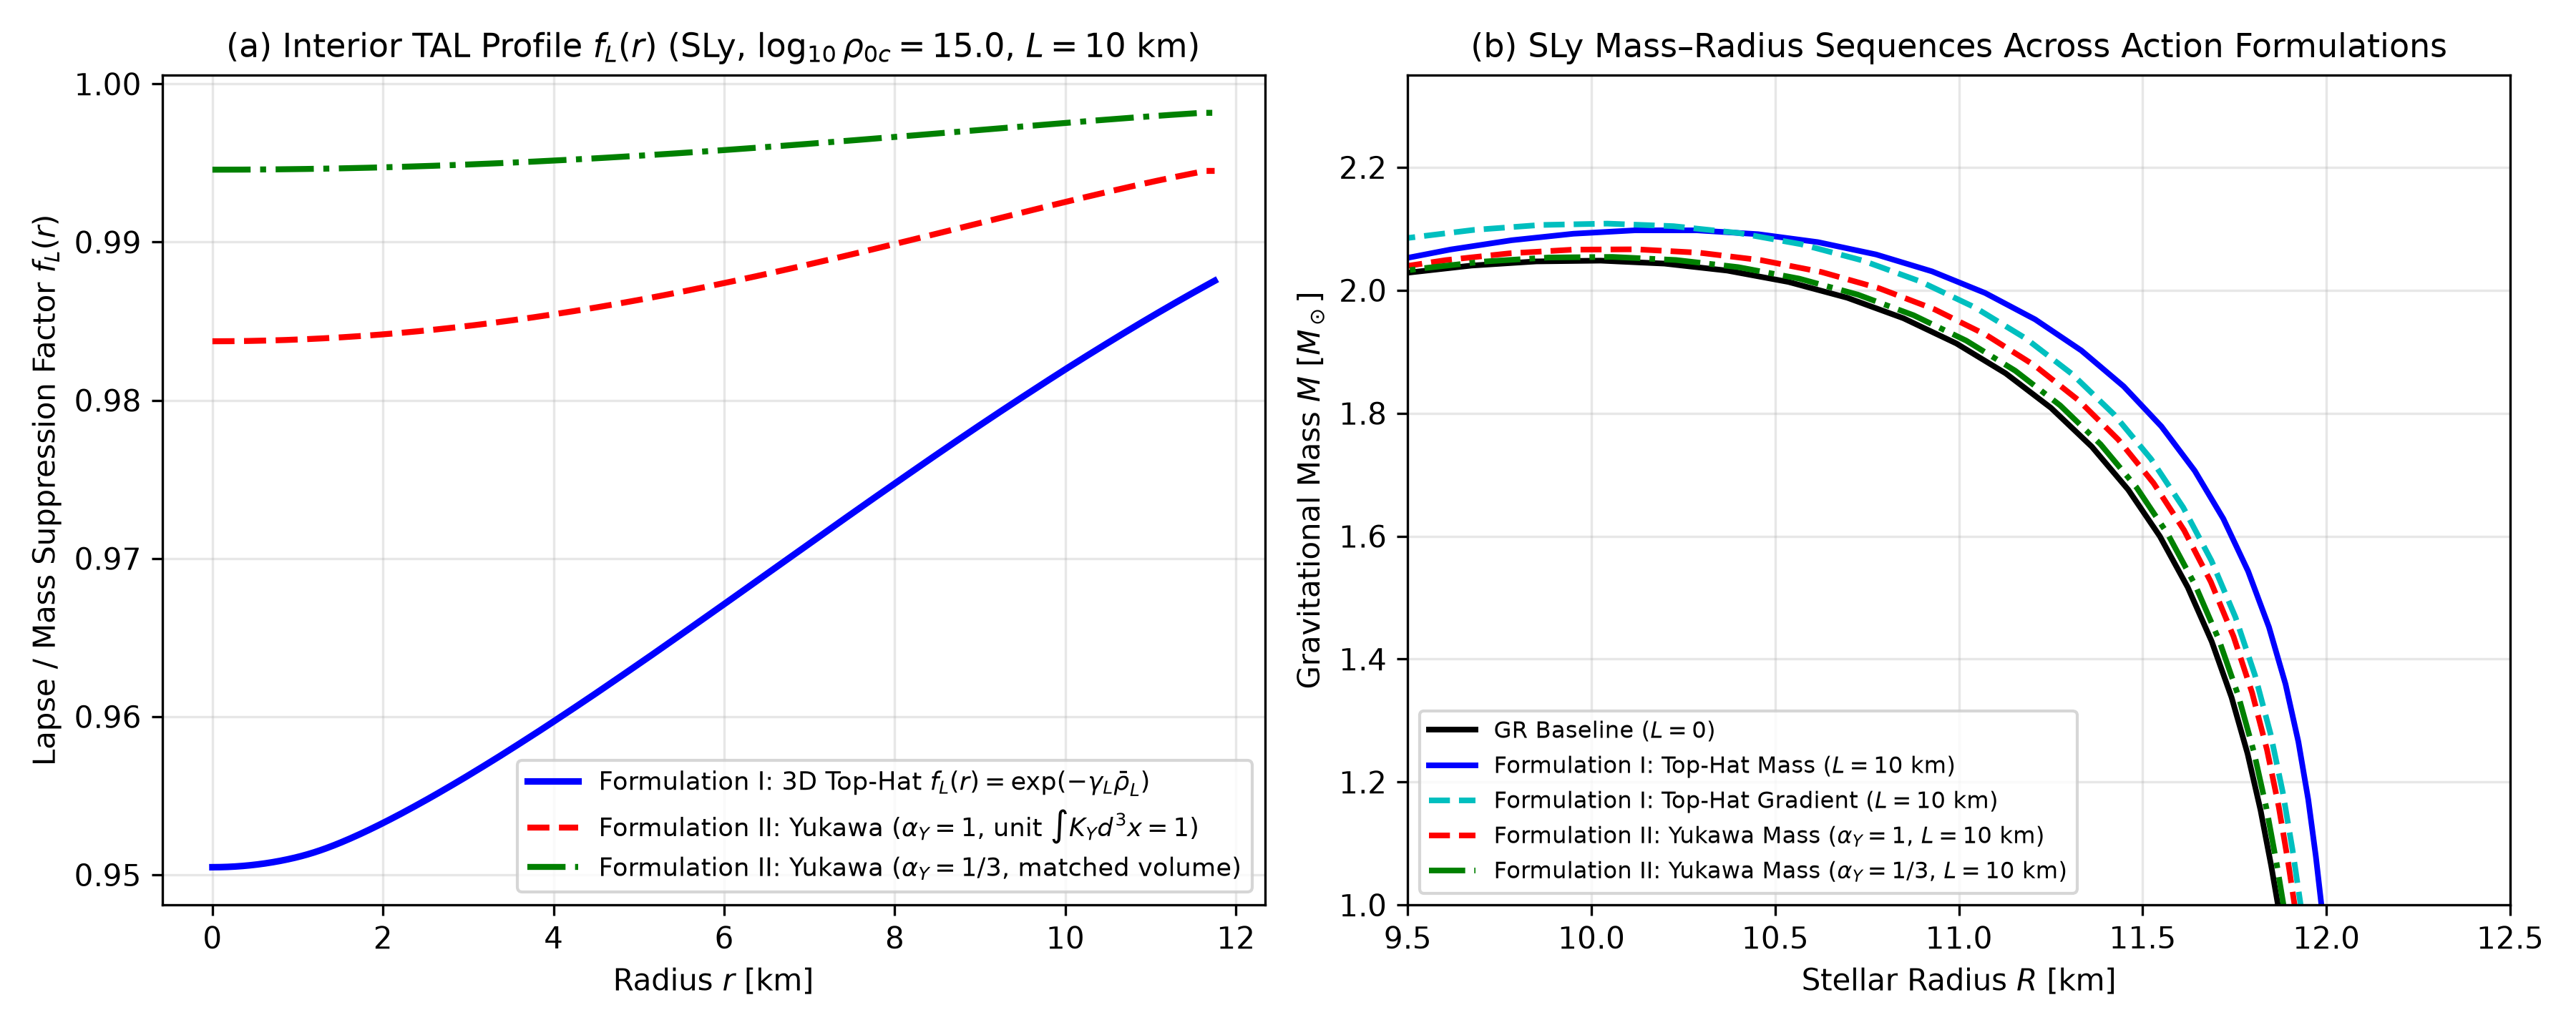
\includegraphics[width=0.66\linewidth]{fig1_action_profiles.png}\vspace{-3mm}
\caption{(a) Belső $f_L(r)$ elnyomási profil $\log_{10}\rho_{0c}=15{,}0$-nál és (b) SLy tömeg--sugár görbék $L=10\,\text{km}$-nél az I.\ megfogalmazás (3D top-hat) és a II.\ megfogalmazás (árnyékolt Yukawa, $\alpha_Y=1$ és $\alpha_Y=1/3$) összevetésével.}
\end{figure}

\section{A V21-háttér statikus nemlokális érintőmodellje és kvázi-dinamikus BVP-tesztje}
A V21 tanulmányban (DOI \texttt{10.5281/zenodo.23602501}) a radiális stabilitást két közelítő, \emph{befagyasztott $f_L$-ű} ($\delta f_L = 0$) Sturm--Liouville-operátorral (\texttt{matter} és \texttt{metric}) vizsgáltam. Annak megértéséhez, hogy miért tér el mindkét befagyasztott $f_L$-ű operátor a $dM/d\rho_c = 0$ statikus tömegmaximumtól, először \texttt{SymPy}-ban meghatároztam a befagyasztott $f_L$-ű Chandrasekhar-féle $\mathcal{L}_{\text{SL}}^{\text{matter}}[\xi]$ operátor és a linearizált $\mathcal{H}_{\text{lin}}[\xi] = (\delta P)' + (\delta\varepsilon+\delta P)\nu' + (\varepsilon+P)\delta\nu'\big|_{\delta f_L=0}$ hidrosztatikai operátor egzakt különbségét tömeg-módban:
\begin{equation}
  \mathcal{L}_{\text{SL}}^{\text{matter}}[\xi] - \sqrt{\frac{r}{r-2m}}\,e^{2\nu}\,\mathcal{H}_{\text{lin}}[\xi]\Big|_{\delta f_L=0} = \frac{4\pi r^{5/2}(f_L - 1)\Gamma P \varepsilon e^{2\nu}}{(r - 2m)^{5/2}}\Big[(4\pi r^3 P - 3r + 7m)\xi - r(r-2m)\xi'\Big]. \label{eq:factored_diff}
\end{equation}
A \eqref{eq:factored_diff} kifejezés $f_L = 1$ (GR) esetén azonosságszerűen eltűnik, mivel a Chandrasekhar-féle parciális integrálás a GR-beli $\lambda' + 2\nu' = 8\pi r e^\lambda(\varepsilon+P)$ Einstein-azonosságot helyettesíti be. Ha azonban $f_L \ne 1$, akkor $\lambda' + 2\nu' = 8\pi r e^\lambda(f_L\varepsilon + P)$, ami előállítja a \eqref{eq:factored_diff}-beli $(f_L-1)$ maradéktagot, RÁADÁSUL elhagyja a $\delta f_L[\delta\varepsilon,\xi]$ nemlokális perturbációt.

A csatolt rendszert (a V21 \texttt{dense\_profile} háttér körül, nem az új ágak körül) a $\delta h(r) = \delta P/(\varepsilon+P)$ entalpiaperturbációra és a $\delta m(r)$ tömegperturbációra linearizálom a szakaszonkénti politróp egzakt $r_{\text{trans}}$ átmeneti sugaraihoz illesztett rácson, beépítve a nemlokális mag-perturbációs operátort:
\begin{equation}
  \delta f_L(r_i) = -\gamma_L f_L(r_i)\sum_j K_{ij}\,\frac{\varepsilon(r_j)+P(r_j)}{c_s^2(r_j)}\,\delta h(r_j), \qquad
  \begin{cases}
    \dfrac{d(\delta h)}{dr} = -\delta\nu'\!\left[\delta h, \delta m, \delta f_L[\delta h]\right] + \omega_0^2\,e^{\lambda-2\nu}\xi, \\[4pt]
    \dfrac{d(\delta m)}{dr} = 4\pi r^2\!\left[f_{\text{mass}}\frac{\varepsilon+P}{c_s^2}\delta h + \varepsilon\,\delta f_{\text{mass}}[\delta h]\right].
  \end{cases} \label{eq:coupled_bvp}
\end{equation}
$\omega_0^2 = 0$-nál a \eqref{eq:coupled_bvp} rendszer pontosan a statikus egyensúlyi egyenletek $\log_{10}\rho_{0c}$ szerinti érintőoperátora. Mint a 2.\ táblázat és a 3.\ ábra mutatja, a \eqref{eq:coupled_bvp} csatolt sajátérték-feladat megoldása az SLy $L=10\,\text{km}$ sorozatok mentén $\sim 7\times 10^{-5}\,\text{dex}$-re ad zérushelyet a $dM/d\rho_c=0$ ponttól (a tiszta GR diszkretizációs alapérték $7{,}12\times 10^{-5}\,\text{dex}$). Mivel $\omega_0^2=0$-nál a feladat $\mathcal{H}_{\text{lin}}[\delta h]=0$-ra redukálódik, ez az egyezés a \emph{statikus} nemlokális linearizációt igazolja, nem a dinamikai tehetetlenséget: a $W\to 4W$ skálázás $\log_{10}\rho_{0c}=15{,}30427$-nél $\omega^2_{4W}/\omega^2_W = 0{,}2500$ arányt ad ($\omega^2_W=4{,}897\times 10^{6}\,\text{s}^{-2}$), azonos $F(0)=0{,}023252$ lövőfüggvény mellett, így a zérushely tehetetlenség-invariáns. A nyers BVP $W$ mátrix nem szimmetrikus; a szimmetrizált Galerkin-alak $\mathbf{M}_{\text{sym}} = \mathbf{D}^{T}\mathrm{diag}(w\,\Delta r)\mathbf{D}$ szimmetrikus, $\min\mathrm{diag}\,\mathbf{M}_{\text{sym}} = 5{,}68\times 10^{-9}>0$; ez Gram-mátrix-tulajdonság, nem a fizikai kinetikus Hesse-mátrix pozitív definitségének bizonyítéka. Az \texttt{omega0\_sq\_sym\_tangent\_s2} oszlop az elsőrendű érintő-becslést ($\omega^2\simeq -F(0)/F'(0)$) adja.

\begin{table}[ht!]
\centering
\caption{Radiális stabilitási zérushely-sűrűségek ($\omega_0^2 = 0$) és a $dM/d\rho_c = 0$ statikus fordulópont összevetése az SLy sorozatokon ($L=0$ GR és $L=10\,\text{km}$ \texttt{mass} és \texttt{gradient} módban) a \texttt{coupled\_stability\_results.csv} és \texttt{conservation\_Residuals.json} alapján.}
\vspace{2pt}
\resizebox{\linewidth}{!}{%
\begin{tabular}{@{}lcccccc@{}}
\toprule
Sorozat & Statikus fordulópont & Befagy.\ $f_L$ \texttt{matter} & Befagy.\ $f_L$ \texttt{metric} & Befagy.\ $f_L$ BVP & \textbf{Statikus érintőmodell (V21-háttér)} & Eltérés-csökkenés \\
(SLy EOS) & $\log_{10}\rho_{0c}$ ($dM/d\rho_c=0$) & $\Delta\log_{10}\rho_{0c}$ [dex] & $\Delta\log_{10}\rho_{0c}$ [dex] & $\Delta\log_{10}\rho_{0c}$ [dex] & $\mathbf{\Delta\log_{10}\rho_{0c}}$ \textbf{[dex]} & Faktor (\texttt{matter} / BVP) \\
\midrule
GR ($L=0\,\text{km}$)           & $15.302445$ & $+2.91\times 10^{-7}$ & $+2.91\times 10^{-7}$ & $+7.12\times 10^{-5}$ & $\mathbf{+7.12\times 10^{-5}}$ & Alapvonal ($f_L \equiv 1$) \\
Mass ($L=10\,\text{km}$)        & $15.308269$ & $-1.34\times 10^{-3}$ & $+1.64\times 10^{-2}$ & $-4.06\times 10^{-3}$ & $\mathbf{+6.97\times 10^{-5}}$ & $\mathbf{19.2\times} \;/\; \mathbf{58.3\times}$ ($235.3\times$ vs.\ \texttt{metric}) \\
Gradient ($L=10\,\text{km}$)    & $15.298753$ & $-3.57\times 10^{-3}$ & $-3.17\times 10^{-4}\;^*$ & $-4.39\times 10^{-3}$ & $\mathbf{+7.39\times 10^{-5}}$ & $\mathbf{48.3\times} \;/\; \mathbf{59.3\times}$ (pozitív súly!) \\
\bottomrule
\end{tabular}}\par\vspace{1pt}
{\scriptsize $^*$Gradiens-módban $L=10\,\text{km}$-nél a közelítő befagyasztott $f_L$-ű \texttt{metric} operátor súlya a felszín közelében indefinitté válik ($\mathcal{W}(r)\le 0$); a \eqref{eq:coupled_bvp} statikus érintőmodell pozitív Gram-súlyt használ (ez nem a kinetikus pozitivitás bizonyítéka).}
\end{table}

\begin{figure}[ht!]
\centering
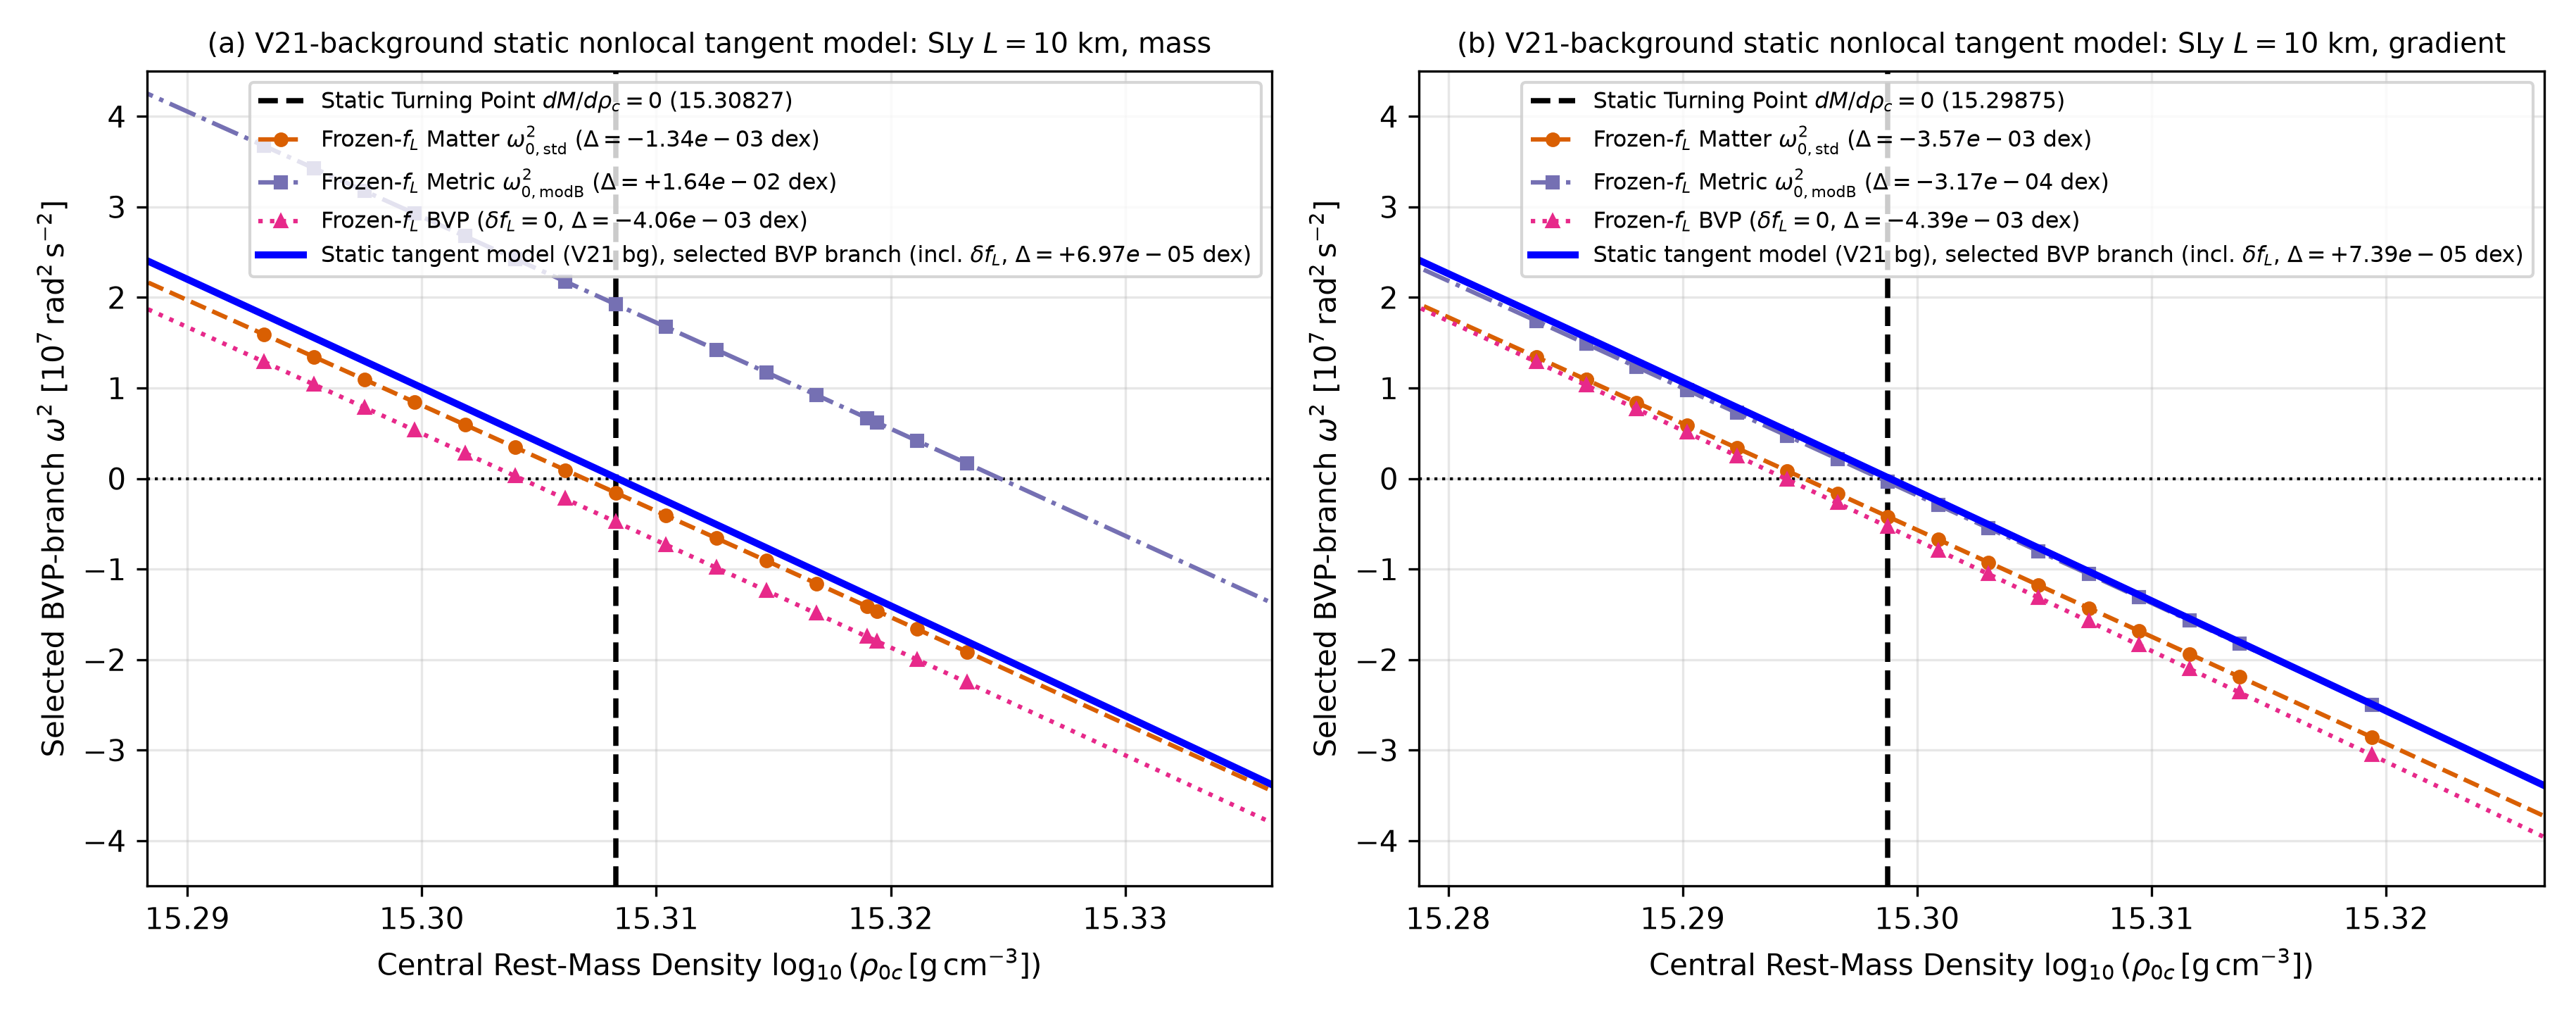
\includegraphics[width=0.66\linewidth]{fig2_coupled_stability.png}\vspace{-3mm}
\caption{A V21-háttér statikus nemlokális érintőmodellje: a kiválasztott BVP-ág $\omega^2(\rho_{0c})$ sajátértéke menete a $dM/d\rho_c = 0$ statikus fordulópont környezetében SLy $L=10\,\text{km}$-re (a) \texttt{mass} és (b) \texttt{gradient} módban, a három befagyasztott $f_L$-ű operátor és a statikus érintőmodell (V21-háttér) összevetésével.}
\end{figure}

\section{Mikroszkopikus óra- és fotoncsatolás a hatásból (H0 vs.\ H1)}
A kovariáns hatás-keretrendszer világossá teszi, mi dönti el a \textbf{H0} és \textbf{H1} megfigyelési hipotézisek közötti választást az atomórák és csillagászati színképvonalak esetén. Jelölje $\Psi_{\text{atomic}} = (\psi_e, A_\mu)$ a barionos közeg $u^\mu$ négyes-sebességével együttmozgó atomóra Dirac-elektron- és Maxwell-elektromágneses mezőit, amelyek a $\tilde{g}_{\mu\nu}[\phi_L]$ effektív Jordan-keretbeli metrikához csatolódnak:
\begin{itemize}\setlength{\itemsep}{1pt}\setlength{\parskip}{0pt}
  \item \textbf{Minimális / tisztán segédmezős csatolás ($\tilde{g}_{\mu\nu} = g_{\mu\nu}$ a $\Psi_{\text{atomic}}$ szektorra $\implies$ H0 hipotézis):} Ha $\phi_L$ kizárólag a makroszkopikus barionos folyadék feszültség-energia tenzorához csatolódik, míg az atomi elektronok és fotonok a fizikai $g_{\mu\nu}$ téridő-metrikán mozognak, akkor az $r = R_*$ felszínen nyugvó atomóra sajátideje $d\tau_{\text{clock}} = \sqrt{-g_{00}(R_*)}\,dt = e^{\Phi_{\text{eff}}(R_*)/c^2}dt$. A felszíni vöröseltolódás tisztán metrikus ($1+z_{\text{H0}} = e^{-\Phi_{\text{eff}}(R_*)/c^2}$), közvetlen $f_L(R_*)$ szorzó nélkül.
  \item \textbf{Univerzális diszform lapse- vagy konform Jordan-csatolás ($\tilde{g}_{\mu\nu} = g_{\mu\nu} + \frac{1 - f_L^2(\phi_L)}{c^2}u_\mu u_\nu$ $\implies$ H1 hipotézis):} Ha az atomórák a $\tilde{g}_{\mu\nu}$ diszform metrikát érzékelik, amelynek együttmozgó idő-idő komponense $g_{00}=-1$, $u_0=-c$ mellett $\tilde{g}_{00} = -1 + (1-f_L^2) = -f_L^2$ (\texttt{SymPy}: \texttt{sym\_disformal\_g00\_residual} $=0$), akkor az atomi átmenet sajátidő-eleme $d\tilde{\tau}_{\text{clock}} = f_L(R_*)\,e^{\Phi_{\text{eff}}(R_*)/c^2}dt$. A végtelenbe futó fotonok koordináta-frekvenciája megmarad, így megjelenik a közvetlen felszíni óraszorzó: $1+z_{\text{H1}} = e^{-\Phi_{\text{eff}}(R_*)/c^2}\,f_L(R_*)^{-1}$.
\end{itemize}
A 3.\ táblázat összefoglalja a \texttt{clock\_coupling\_H0\_H1.csv}-ben kapott numerikus előrejelzéseket a Sirius B ($M=1{,}018\,M_\odot$, $R_*=5586{,}5\,\text{km}$, $n=3$ politróp) és a V20 $8558\,\text{kg}$-os mozgatható gránitkamra ($\rho=2750\,\text{kg/m}^3$, $V_{\text{tot}}=3{,}1120\,\text{m}^3$) esetére. Mivel a Sirius B még H1 alatt is szabadon hagyja az $L \lesssim 10^6\,\text{m}$ tartományt, mind a H0, mind a H1 életképes marad neutroncsillag- ($L \sim 1\text{--}10\,\text{km}$) és laboratóriumi ($L \sim 1\,\text{m}$) skálán; a V20 gránitkamra közvetlenül a H1 óra-ágat teszteli $|\Delta y_{\text{H1}}| = 1{,}436\times 10^{-24}$ ($L=1{,}0\,\text{m}$) szinten.

\begin{table}[!tb]
\centering
\caption{A hatásból levezetett \textbf{H0} ($\tilde{g}_{\mu\nu}=g_{\mu\nu}$) és \textbf{H1} (diszform lapse $\tilde{g}_{00}=f_L^2 g_{00}$) óracsatolások kvantitatív összehasonlítása a Sirius B ($n=3$) és a V20 $8558\,\text{kg}$-os gránitkamra esetén (\texttt{clock\_coupling\_H0\_H1.csv}).}
\vspace{2pt}
\resizebox{\linewidth}{!}{%
\begin{tabular}{@{}lrrrrrrr@{}}
\toprule
Rendszer & $L$ [m] & $f_L(R_*)$ Top-Hat & $f_L(R_*)$ Yukawa & H0 előrejelzés & H1 Top-Hat előrej. & H1 Yukawa előrej. & Egység \\
\midrule
Sirius B ($1{,}018\,M_\odot$) & $1.0\times 10^3$ & $1.000000$ & $1.000000$ & $80.70055$ & $80.70055$ & $80.70055$ & km/s \\
Sirius B ($1{,}018\,M_\odot$) & $1.0\times 10^4$ & $1.000000$ & $1.000000$ & $80.70055$ & $80.70055$ & $80.70055$ & km/s \\
Sirius B ($1{,}018\,M_\odot$) & $1.0\times 10^6$ & $1.000000$ & $1.000000$ & $80.69839$ & $80.70094$ & $80.74476$ & km/s \\
Sirius B ($1{,}018\,M_\odot$) & $5.0\times 10^6$ & $0.999984$ & $0.999993$ & $80.69487$ & $85.38911$ & $82.85137$ & km/s \\
\midrule
V20 gránit ($8558\,\text{kg}$) & $0.50$ & $1.000000$ & $1.000000$ & $+3.075\times 10^{-48}$ & $-3.318\times 10^{-25}\;(-3.318\times 10^{-25})$ & $-2.008\times 10^{-25}\;(-1.943\times 10^{-25})$ & $\Delta y$ \\
V20 gránit ($8558\,\text{kg}$) & $0.85$ & $1.000000$ & $1.000000$ & $+1.208\times 10^{-47}$ & $-1.303\times 10^{-24}\;(-1.303\times 10^{-24})$ & $-3.373\times 10^{-25}\;(-3.101\times 10^{-25})$ & $\Delta y$ \\
V20 gránit ($8558\,\text{kg}$) & $1.00$ & $1.000000$ & $1.000000$ & $+1.331\times 10^{-47}$ & $-1.436\times 10^{-24}\;(-1.436\times 10^{-24})$ & $-3.781\times 10^{-25}\;(-3.407\times 10^{-25})$ & $\Delta y$ \\
\bottomrule
\end{tabular}}\par\vspace{1pt}
{\scriptsize V20 sorok: H0 oszlop = a newtoni GR feletti TAL-többlet IN ($\mathbf{r}=\mathbf{0}$) állásban; H1 oszlopok = IN-eltolódás (IN$-$OUT differenciális jel, $D_{\text{out}}=2{,}0\,\text{m}$). Newtoni GR: $\Phi_N(\text{IN})/c^2 = -9{,}269\times 10^{-24}$, IN$-$OUT $= -6{,}094\times 10^{-24}$; a $\sigma_y=10^{-18}$ szemléltető referenciaérték. Szíriusz B közös effektívtömeg-proxyn (rögzített $n=3$ Lane--Emden-profil a H0 effektívtömeg-eltolással, nem újonnan megoldott egyensúly) $L=10^3\,\text{km}$-nél: H0 $80{,}69839$, H1 top-hat $80{,}69878\,\text{km/s}$.}
\end{table}

\noindent{\scriptsize\color{slate}\textbf{Archív hivatkozások:} Szabolcsi D., Zenodo DOI-k: \texttt{10.5281/zenodo.23217189} (V14), \texttt{10.5281/zenodo.19666220} (V17), \texttt{10.5281/zenodo.23497128} (V19), \texttt{10.5281/zenodo.23540741} (V20), \texttt{10.5281/zenodo.23602501} (V21) és \texttt{10.5281/zenodo.23604423} (V22 Book Edition).}

\end{document}
